\thispagestyle{plain}
\section{Metode}
\pagestyle{headings}
Hvis man ser på en række vesikler, er det tydeligt at de ikke er ens. De har forskellig størrelse, både i kantens tykkelse og i diameteren. To eksempler på vesikler er vist i figur \ref{fig:premethod_daddy}, hvor det fremgår at de begge er relativt cirkulære. At vesiklerne er meget forskellige fremgår også tydeligt af figuren. Selvom begge har nogenlunde samme farve kant har vesiklen til venstre et meget lyst indre, hvor vesiklen til højre er meget mørkere. 

I introduktionen nævnte vi hvor meget støj der var omkring alle vesiklerne, og hvordan det derfor var svært at se overgangen i kanterne. Vi forsøger derfor med en form for udglatning af billedet for at undertrykke støjen, og samtidig også et filter der kan fremhæve de interessante værdier.

\begin{figure}[H]
	\centering
	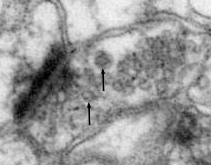
\includegraphics[scale=3.5]{files/premethod/img/ves_color_daddy.png}
	\caption{Dette er cellen hvorfra vi tager to vesikler.\label{fig:premethod_daddy}}
\end{figure}

At vesiklerne har fællestræk men alligevel er så forskellige, antyder at en enkelt metode ikke vil finde alle vesiklerne, og at vi i stedet skal kombinere flere metoder der tilsammen kan finde alle typer af vesikler.

Det faktum at nogen af vesiklerne er relativt cirkulære, giver os ideen at detektere cirkler i billedet. Til dette benytter vi os af Hough-cirkeldetektion. Metoden er forklaret nærmere i afsnit \ref{premethod_hough}, men for at metoden kan fungere, skal billedet behandles først. Her benytter vi et Gaussfilter der udglatter billedet før et Sobelfilter finder retninger i billedet som en kantdetektor bruger til at finde hvor der er kanter i billedet. Hver af disse funktioner er forklaret nærmere nedenfor, og vi vil til slut evaluere på resultatet.

Vi vil benytte celleudsnittet i figur \ref{fig:premethod_daddy}, uden pilene, til at finde vesikler i. Billedet er et godt eksempel da det både indeholder støj, vesikler og en kant på cellen hele vejen rundt.

\subsection{Gaussisk udglatning}\label{sec:premethod_gaussblur}
En gaussisk udglatning er et lavpasfilter da funktionen i virkeligheden reducerer billedets højfrekvente værdier. Filteret bliver typisk brugt til at reducere billedstøj og udglatte områder. 

\begin{figure}[H]
	\begin{minipage}[b]{0.5\linewidth}
		\centering
		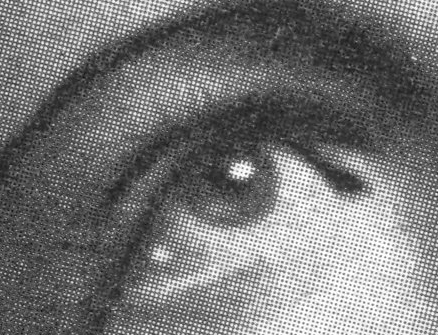
\includegraphics[scale=1.5]{files/premethod/img/gauss_pre.png}
	\end{minipage}
	\hspace{0.5cm}
	\begin{minipage}[b]{0.5\linewidth}
		\centering
		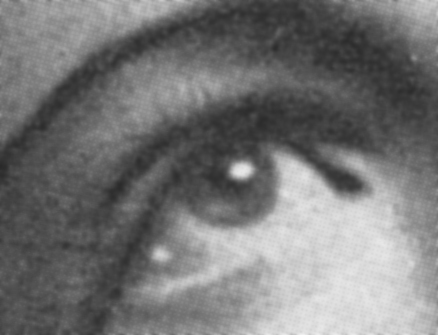
\includegraphics[scale=1.5]{files/premethod/img/gauss_post.png}
	\end{minipage}
	\caption{Billede før og efter en Gauss udglatning\cite{gaussblur}.\label{fig:premethod_gauss}}
\end{figure}

I figur \ref{fig:premethod_gauss} ses to billeder hvor det første er originalbilledet og det andet er billedet der er blevet behandlet med gaussfilter. Resultatet er tydeligt, billedet er glattere og med mindre støj. I to dimensioner er en gaussisk funktion givet ved: 
\begin{align}
	G(x,y) = \frac{1}{2\pi\sigma^2}e^{-\frac{x^2+y^2}{2\sigma^2}}\label{ali:premethod_gaussG}\cite{gauss}
\end{align}
hvor x er distancen fra origo på den horisontale akse, y er distancen fra origo på den vertikale akse og $\sigma$ er standard afvigelsen af den gaussike fordeling. 
%Når man omtaler størrelsen på den gaussiske kerne er det størrelsen på dimensionen for $G$ der bygges. Ser vi på (\ref{ali:premethod_gaussG}) så er det kun eksponentialdelen der ændrer sig når x og y ændres. Vi ser så at et større x og y får eksponentialdelen til at gå mod 0. At hæve $\sigma$ værdien vil betyde at eksponentialdelen går langsommere mod 0. Der er ikke nogen grund til at lave en matrice med den gaussiske fordeling større end dens indgange har værdier på tal større end 0. 
Da vi er ude efter at udglatte billeder med vesikler hvis kant har en bredde på ca. 7 pixels, vælger vi derfor $\sigma$ værdien 7.

I figur \ref{fig:premethod_GaussCelle} ses vores cellebillede fra figur \ref{fig:premethod_daddy} der er blevet behandlet med et gaussfilter. Det er tydeligt at billedet er blevet udglattet, men det er samtidig også blevet sværere at se overgangen mellem vesiklerne. Dette er ikke et positivt resultat og vi forkaster funktionen.

\begin{figure}[H]
	\centering
	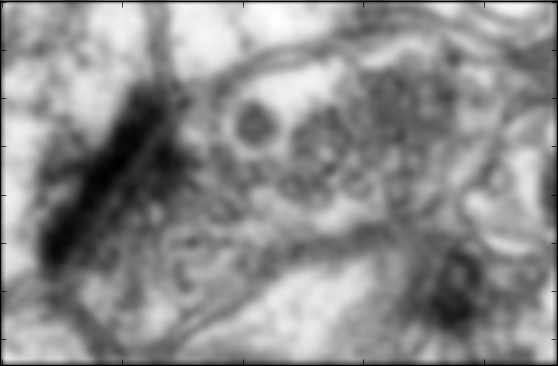
\includegraphics[scale=0.8]{files/premethod/img/gausscell.png}
	\caption{Celleudsnit behandlet med et gaussfilter med $\sigma$ værdi 7.\label{fig:premethod_GaussCelle}}
\end{figure}

\subsection{Sobelfilter og kantdetektion}
I billedbehandling benyttes Sobeloperatoren især i kant detektion\cite{edge}. Operatoren udregner gradienten for hvert punkt i billedet. Gradienten er retningsændringen i intensitet eller farve i et billede. Det resulterende billede indeholder så retningen i den størst mulige ændring fra mørk til lys. Jo større intensitetsforskel der er mellem to tilstødende pixelgrupper des større er sandsynligheden for at der findes en kant mellem disse to grupper\cite{imggrad}. Et eksempel på et billede der er blevet behandlet med et sobelfilter ses i figur \ref{fig:premethod_sobelres}.


\begin{figure}[H]
	\begin{minipage}[b]{0.5\linewidth}
		\centering
		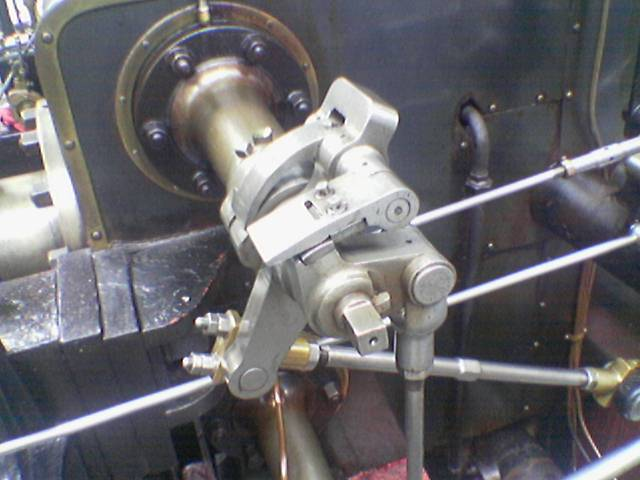
\includegraphics[scale=0.25]{files/premethod/img/sobel1.PNG}
	\end{minipage}
	\hspace{0.5cm}
	\begin{minipage}[b]{0.5\linewidth}
		\centering
		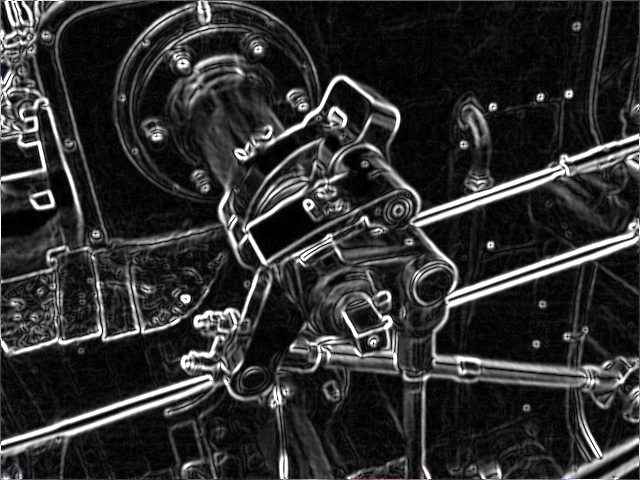
\includegraphics[scale=0.25]{files/premethod/img/sobel2.PNG}
	\end{minipage}
	\caption{Originalbilledet til venstre\cite{sobel1}, og behandlet med et Sobelfilter til højre\cite{sobel2}.\label{fig:premethod_sobelres}}
\end{figure}

Det er ikke specielt beregningstungt at behandle et billede med et sobelfilter da operatoren baserer sig på at folde billedet med et lille separabel heltalsfilter først i horisontal og derefter i vertikal retning\cite{sobel}. Hver af filtrene repræsenterer sin egen retning, så $G_x$ er defineret som hvordan gradienten ændrer sig i højregående retning, og $G_y$ er hvordan gradienten ændrer sig i nedadgående retning. $G_x$ og $G_y$ defineret i  (\ref{ali:premethod_sobelG}), hvor $I$ repræsenterer originalbilledet der foldes med, og $*$ operatoren betyder foldning.

\begin{align}
	G_y = \begin{bmatrix}
		-1 & -2 & -1\\
		0 & 0 & 0\\
		1 & 2 & 1
	\end{bmatrix} * I
	&&
	G_x = \begin{bmatrix}
		-1 & 0 & 1\\
		-2 & 0 & 2\\
		-1 & 0 & 1
	\end{bmatrix} * I
	\label{ali:premethod_sobelG}
\end{align} 

Det resulterende Sobelbillede fås ved formlen 
\begin{align}
	G = \sqrt{G_x^2 + G_y^2}
\end{align}

På ethvert tidspunkt kan vi så finde retningen som kanten har i enhver pixel ved 
\begin{align}
	\Theta = \arctan\left(\frac{G_y}{G_x}\right)
	\label{ali:premethod_sobelTheta}
\end{align}
hvor $\Theta$ er 0 for en vertikal kant med mørkt på den venstre side. Vi skal bruge disse formler senere når vi ser på Hough cirkel detektionen der kan benytte sig af Sobelfilteret når der skal findes kanter. 

\begin{figure}[H]
	\centering
	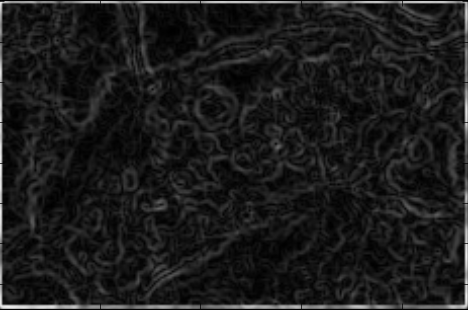
\includegraphics[scale=0.8]{files/premethod/img/sobel3.png}
	\caption{Originalbilledet foldet med et Sobelfilter.\label{fig:premethod_sobel}}
\end{figure}

Det resulterende Sobelbillede vil kun fremstå med værdi større end 0 i de pixels man med stor tiltro mener er en kant. Originalbilledet fra figur \ref{fig:premethod_daddy} foldet med Sobelfilteret ses i figur \ref{fig:premethod_sobel}. 

Dette er ikke noget særlig godt billede da kanterne omkring vesiklerne ikke fremstår tydeligere end støjen. Vi havde håbet på en kant der fremstod klart lysere end resten så vi med en tærskelværdi kunne isolere disse kanter. Vi har alligevel påført en tærskelværdi på 40 på billedet, og resultatet ses i figur \ref{fig:premethod_sobel}.

\begin{figure}[H]
	\centering
	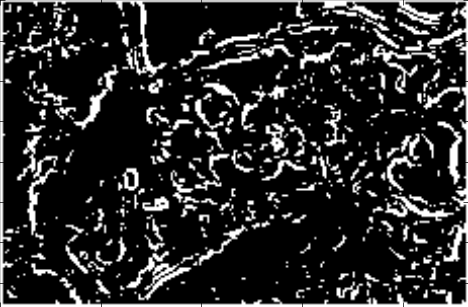
\includegraphics[scale=0.8]{files/premethod/img/edgemap2.png}
	\caption{Sobelfilteret fra figur \ref{fig:premethod_sobel} med en tærskelværdi på 40.\label{fig:premethod_edgemap}}
\end{figure}

Her er det stadig tydeligt at der er meget andet støj end de vesikler der skal detekteres. Hvis vi ændrer tærskelværdien vil noget af støjen forsvinde, men det samme vil vesiklerne selv, så dette er ikke en mulighed.

Men hvad er så grunden til dette dårlige resultat? Vi omtalte kort at vesiklerne i figur \ref{fig:premethod_daddy} har forskelligt farvet indre. I figur \ref{fig:premethod_vescolors} har vi indtegnet 3 pile til hver vesikel. Den ene pil peger på vesiklens indre, og de to andre peger på to steder på kanten af vesiklen.  Figuren illustrerer hvorledes to forskellige vesikler kan have vidt forskellig karakteristika på trods af at de er taget fra samme celle.

% Tager vi vesiklen til venstre, ses det at der er stor intensitetsforskel på vesiklens indre, og kanten af vesiklen. Det lyseste sted på kanten har stadig en intensitetsværdi på 33 lavere end centrum. En overgang fra kant til centrum er her derfor meget tydelig. Det bemærkes dog også at der er en intensitetsværdi på 35 på det mørkeste og lyseste sted på kanten af vesiklen. 
% 
% Tager vi så vesiklen til højre, ser vi at der er en intensitetsværdi på 2 fra det lyseste sted på kanten til det mørkeste. Dette er altså meget det samme som den første vesikel, og intensitetsværdierne ligger da også meget tæt (132 versus 122 for lyseste og 97  versus 89 for det mørkeste). 

\begin{figure}[H]
	\centering
	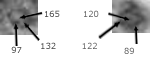
\includegraphics[scale=5]{files/premethod/img/ves_colors2.png}
	\caption{Problematikken med forskellig intensitetsværdi i vesiklernes indre illustreret.\label{fig:premethod_vescolors}}
\end{figure}

At der er så stor intensitetsforskel på vesiklerne er dog ikke den eneste udfordring. Kanterne består ikke af rene linjer uden huller imellem. Zoomer man ind på et billede af en vesikel ses det tydeligt at der er store "huller" mellem de mørke pixels der udgør kanten. Dette er nok den største grund til at Sobelfilteret ikke producerer et godt resultat. En anden grund kan være at vesiklerne nogle gange ligger meget tæt, og at der derfor ikke er en overgang fra mørk til lys ved kanterne.

\subsection{Houghdetektion}\label{premethod_hough}
Vi har ikke produceret et særlig godt resultat med vores Sobelfilter, og kan derfor ikke gøre os store forhåbninger om at få et godt resultat med Hough detektionen.

I de tidligere afsnit har vi vist hvordan vi har udglattet billedet, fundet kanter, og gradienten i hvert punkt på disse kanter. Disse resultater vil vi benytte til at estimere vesiklernes centrum. I (\ref{ali:premethod_sobelG}) viste vi $G_x$ og $G_y$ som jo var gradienterne i horisontal og vertikal retning. Vi fandt også $\theta$ i (\ref{ali:premethod_sobelTheta}), der er vinklen på en kant i den givne pixel. Vi har i vores observationer af vesiklerne også fundet ud af at de kan variere i størrelse fra 15x15 pixel, og op omkring 30x30 pixels.

Ideen er at tage hver pixel der menes at ligge på en kant, og tegne en ortogonal linje ud fra dette punkt i et nyt billede. Skæringspunkterne mellem flere linjer kandiderer til at være centrum i en cirkel. Disse punkter kan findes ved at vælge en korrekt tærskelværdi. En af disse linjer ses i figur \ref{fig:premethod_houghLines}. 

\begin{figure}[H]
	\centering
	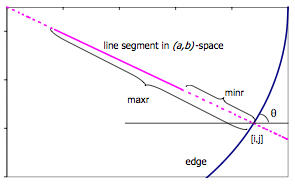
\includegraphics[scale=1]{files/premethod/img/hough_lines.png}
	\caption{Linje tegnet ud fra pixel [i,j] der menes at ligge på en kant\cite{houghrep}.\label{fig:premethod_houghLines}}
\end{figure}

I figur \ref{fig:premethod_houghres} ses 4 billeder. Den første er bare en cirkel vi ønsker at detektere. I det andet billede er så tegnet nogle af de linjer der går igennem punkter på kanten af cirklen. I det tredie billede ses de samme linjer bare tegnet i et nyt billede. I det fjerde og sidste billede fremkommer centrum ved en passende tærskelværdi.

\begin{figure}[H]
	\begin{minipage}[b]{0.5\linewidth}
		\centering
		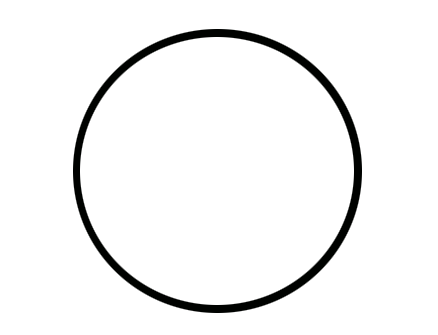
\includegraphics[scale=1.5]{files/premethod/img/dirmap1.png}
	\end{minipage}
	\hspace{0.5cm}
	\begin{minipage}[b]{0.5\linewidth}
		\centering
		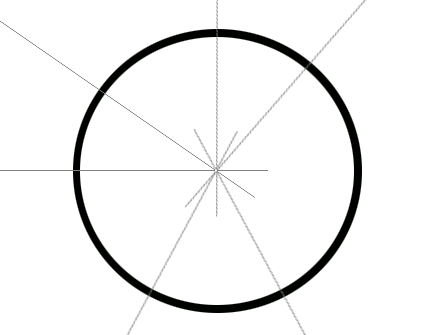
\includegraphics[scale=1.5]{files/premethod/img/dirmap2.png}
	\end{minipage}\\\\
	\begin{minipage}[b]{0.5\linewidth}
		\centering
		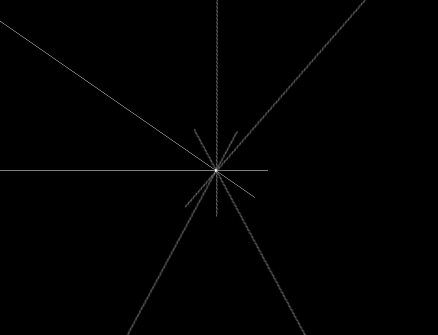
\includegraphics[scale=1.5]{files/premethod/img/dirmap3.png}
	\end{minipage}
	\hspace{0.5cm}
	\begin{minipage}[b]{0.5\linewidth}
		\centering
		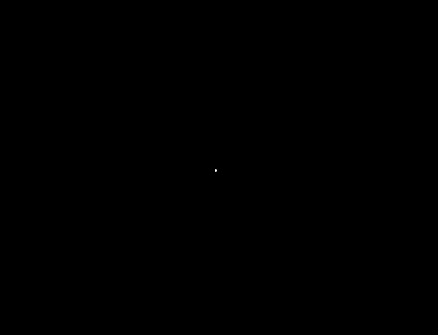
\includegraphics[scale=1.5]{files/premethod/img/dirmap4.png}
	\end{minipage}
	\caption{Øverst venstre: originalt billede. Øverst højre: cirkel med nogen af linjerne tegnet. Nederst venstre: det resulterende billede med nogen af linjerne tegner. Nedest højre: resultat efter tærskelværdi.\label{fig:premethod_houghres}}
\end{figure}

Vi forsøger os så med vores Sobel-behandlede billede fra figur \ref{fig:premethod_edgemap}. Vi tegner linjer ud fra hver af disse punkter med radius mellem 7 og 15. Det resulterende billede ses i figur \ref{fig:premethod_houghCellLines}. 

\begin{figure}[H]
	\centering
	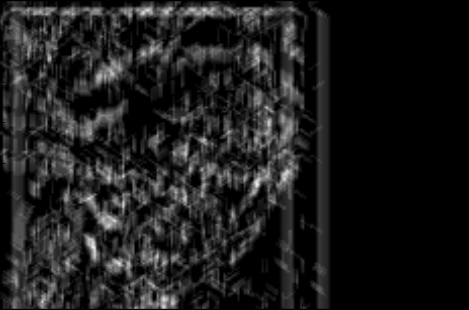
\includegraphics[scale=0.8]{files/premethod/img/houghCell2.png}
	\caption{Houghlinjer tegnet ud fra sobelbilledets kanter.\label{fig:premethod_houghCellLines}}
\end{figure}

Der er mange linjer der er blevet tegnet og det er ret uoverskueligt. Dette var hvad vi forventede da der er så mange kanter på billedet vi behandler. Vi forsøger med en tærskelværdi der kun tegner de pixels der har en intensitetsværdi på over 200. Resultatet påtegnet med rødt på originalbilledet ses i figur \ref{fig:premethod_houghCellLinesThresholdOnOrig}.

Her ses det tydeligt at kun meget få af de røde områder ligger i centrum af en vesikel, mens de fleste ligger langt fra. Som beskrevet i afsnittet om foldning så kan man ikke regne med de yderste pixels i rammen omkring et billede der er blevet foldet. Men selvom man ser bort fra disse virker de røde områder tilfældigt sat i forhold til vesiklerne.

Som vi frygtede får vi altså ikke noget godt resultat ud af Hough-cirkeldetektionen, som kan skyldes at vi giver den et kantbillede der ikke er robust nok. En anden mulighed er at krumningen for en cirklerne ikke er cirkulære nok, så sandsynligheden for at vi vil finde cirkler i billedet er heller ikke særlig stor. En løsning kunne være at afprøve Hough elipsedetektion, men da en vesikel ikke har en generel cirkulær struktur gør vi os ingen forhåbninger om at metoden skulle kunne producere et brugbart resultat.

\begin{figure}[H]
	\centering
	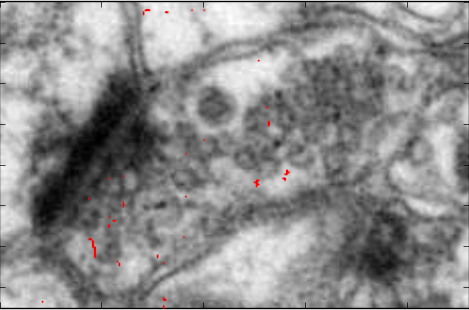
\includegraphics[scale=0.8]{files/premethod/img/houghres2.png}
	\caption{De resulterende områder fundet ved hjælp af Hough-cirkeldetektion plottet med rødt på det originale billede.\label{fig:premethod_houghCellLinesThresholdOnOrig}}
\end{figure}

\subsection{Afledet Gaussfilter}
Vores resultat af Hough-cirkeldetektionen blev ikke særlig godt. Dette skyldes bl.a. at billedet som kantdetektionen producerer indeholder for meget støj, så kanterne ikke fremstår tydelige. En mulig optimering er at benytte et afledet gaussfilter. Ved at bruge det afledte gaussfilter i hver retning, kan vi lave et nyt filter, som fremhæver højderygge i billedet, såsom kanterne på en vesikel. Et simpelt eksempel er vist i figur \ref{fig:premethod_gaussCirc} hvor billedet til venstre er originalbilledet af to figurer. I billedet til højre ses resultatet efter at folde med det nye filter.

\begin{figure}[H]
	\begin{minipage}[b]{0.5\linewidth}
		\centering
		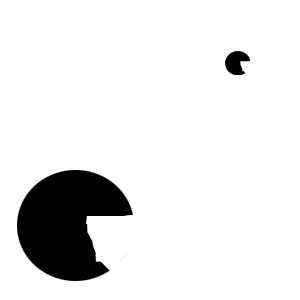
\includegraphics[scale=1.3]{files/premethod/img/gauss_derived_circ1.png}
	\end{minipage}
	\hspace{0.5cm}
	\begin{minipage}[b]{0.5\linewidth}
		\centering
		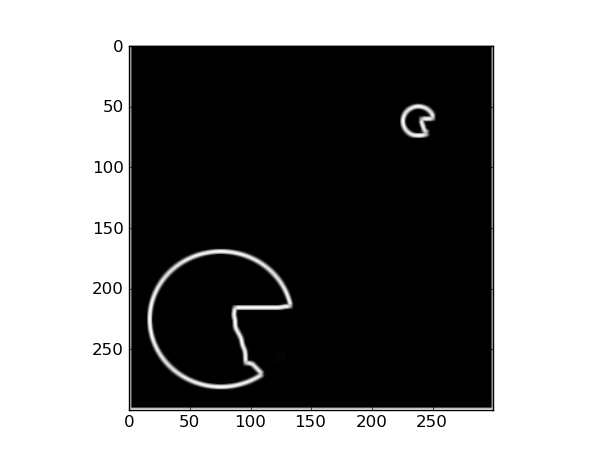
\includegraphics[scale=0.5]{files/premethod/img/gauss_derived_circ2.png}
	\end{minipage}
	\caption{Originalbillede samt det resulterende billede efter foldning med det afledete gaussfilter med $\sigma$ værdi 7.\label{fig:premethod_gaussCirc}}
\end{figure}

Dette er et resultat vi meget gerne vil opnå med vores billeder, da ønskescenariet vil være at få en bedre segmentering af kanterne der kan benyttes af Hough cirkel detektionen.

Vi har at et gaussfilter i to dimensioner er:
\begin{align}
	G(x,y) = \frac{1}{2\pi\sigma^2}e^{-\frac{x^2+y^2}{2\sigma^2}}
\end{align}
og vi har altså at de afledte af gaussfilteret er:
\begin{align}
	G_x(x,y) = \frac{\partial}{\partial x}G(x,y)=-\frac{x}{2\pi\sigma^4}e^{-\frac{x^2+y^2}{2\sigma^2}} \label{ali:premethod_gauss}\\
	G_y(x,y) = \frac{\partial}{\partial y}G(x,y)=-\frac{y}{2\pi\sigma^4}e^{-\frac{x^2+y^2}{2\sigma^2}}
\end{align}

Dette kan vi illustrere grafisk ved nedenstående to plots i figur \ref{fig:premethod_gxgy}, hvor vi kan se at figurene er symmetrisk omkring akserne ligesom Sobelfilterværdierne fra (\ref{ali:premethod_sobelG}). Dette begrunder også ligheden mellem de billeder de to filtre producerer. Den helt store forskel er dog at man med det afledte gaussfilter kan styre størrelsen på standardafvigelsen. 

\begin{figure}[H]
	\begin{minipage}[b]{0.5\linewidth}
		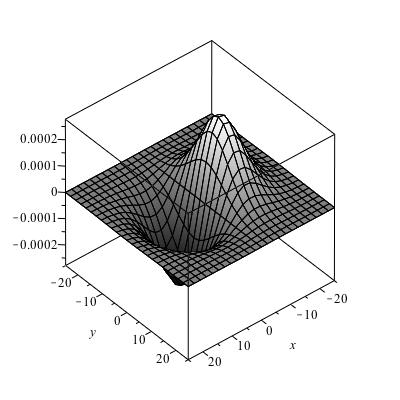
\includegraphics[scale=0.5]{files/premethod/img/g_x.jpg}
	\end{minipage}
	\hspace{0.5cm}
	\begin{minipage}[b]{0.5\linewidth}
		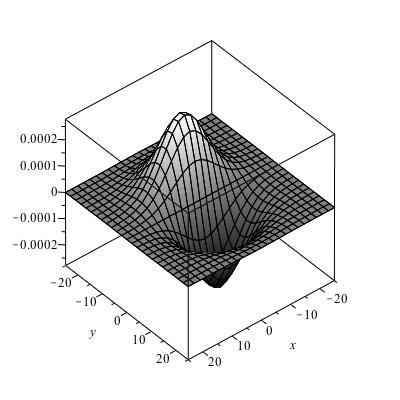
\includegraphics[scale=0.5]{files/premethod/img/g_y.jpg}
	\end{minipage}
	\caption{$G_x$ (venstre) og $G_y$ (højre) plottet med $\sigma$ værdi 7 og x og y værdier fra -25 til 25 med orientation $[$x y z$]$ = $[$50 50 0$]$.\label{fig:premethod_gxgy}}
\end{figure}

Vi finder så vores nye billede ved at folde det originale billede med det afledte gaussfilter i x-retningen, det samme for gaussfilteret afledt i y-retningen og så tage kvadratroden af summen af de kvadrerede resultater.
\begin{align}
	I_x = I * G_x && I_y = I * G_y && I_{ny} = \sqrt{I_x^2+I_y^2}
\end{align} 
hvor $I$ er det originale billede, og $G_x$ hhv. $G_y$ er gaussfilteret afledt i x- hhv. y-retningen.

Vores testcellebillede foldet med dette nye filter med en $\sigma$ på 7 giver resultatet i figur \ref{fig:premethod_gaussCell}. Vi benytter netop denne værdi da kanten på en vesikel netop er 7 pixel bred.
% TAG NYT BILLEDE!
\begin{figure}[H]
	\centering
	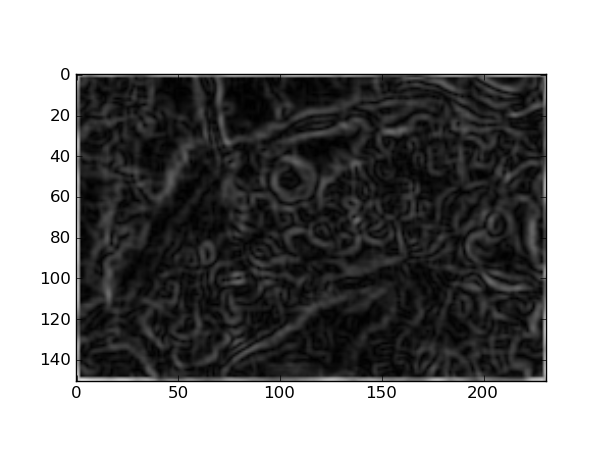
\includegraphics[scale=0.8]{files/premethod/img/gauss_derived_cell2.png}
	\caption{Originalbillede af en celle foldet med det afledete gaussfilter.\label{fig:premethod_gaussCell}}
\end{figure}

Resultatet af dette er ikke godt. Der er stadig alt for meget støj omkring vesiklerne og det er ikke blevet nemmere at se hvor de præcis er. Det er samtidig svært at se en synlig forskel i forhold til resultatet med sobelfilteret. Forskellen er dog, som nævnt ovenfor, at vi her kan styre størrelsen på gausskernen, som f.eks. benyttes i Difference of Gaussians (DoG). Denne vej har vi også afsøgt, men dog uden nævnbart resultat. 

%Dette giver os ideen til Sum of Derived Gaussians beskrevet i næste afsnit.

% \subsection{Sum of derived gaussians}
% Når man folder et billede med et gaussfilter får man et resulterende udglattet billede. Man kan så styre størrelsen på kernen som filteret benytter, hvilket påvirker hvor udglattet billedet bliver. Princippet i Difference of Gaussians (DoG) er at tage to ens gaussfunktioner, kun adskilt af deres kernestørrelse, og trække dem fra hinanden så det giver et nyt filter. Hvis man havde taget det originale billede og foldet med gaussfilteret med en kerne $\sigma_1$ og trukket fra en kopi af det originale billede foldet med gaussfilteret med en kerne $\sigma_2$ så giver det samme resultat som det billedet foldet med DoG filteret. Funktionen viser altså forskellen mellem et billede foldet med gaussfilter med to forskellige kerner. 
% 
% Idet vores cellebillede foldet med det afledte gaussfilter, vist i figur \ref{fig:premethod_gaussCell} ovenfor, er høje værdier omkring de steder hvor der er en kant, ved vi at de pixels har værdier større end 0. Vores ide går så ud på at tage forskellige kerner og folde billedet med det afledte gaussfilter. De resulterende billeder skal så i stedet ligges sammen og på dem måde fremhæve de steder der er kanter. Ved at vælge gausskerner der kun fremhæver dele af vesiklerne og ligge sammen med de kerner der viser et tydeligere billede af vesiklerne, er vores håb at vi vil få et bedre kantbillede.
% 
% \begin{figure}[H]
% 	\centering
% 	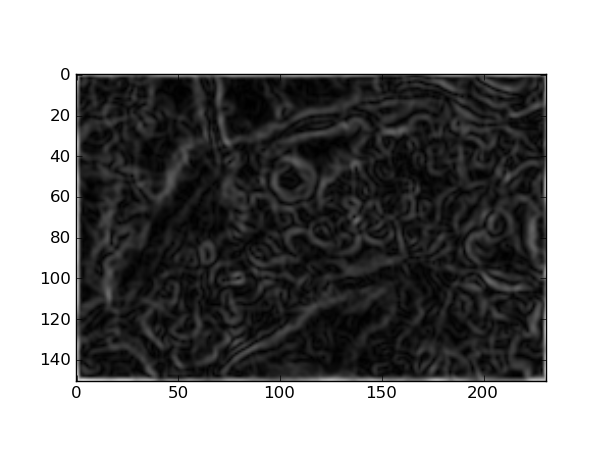
\includegraphics[scale=0.8]{files/premethod/img/sum_der_gauss.png}
% 	\caption{Originalbillede af en celle foldet med filtret Sum Of Derived Gaussians.\label{fig:premethod_sumOfDiff}}
% \end{figure}
% 
% I figur \ref{fig:premethod_sumOfDiff} ses det resulterende billede. Det er dog ikke de store ændringer vi kan se i forhold til resultatet før, og vi gør os derfor ikke større forhåbninger for at Hough cirkel detektionen skal opnå bedre resultater.

\subsection{Foldning med kantkonkur efter vesikelbillede}
Da vi ikke har haft held til at finde vesikelkanter udelukkende ved brug af filtre, vil vi nu i stedet prøve at finde det ved hjælp af en form for matchene billeder. Vores første metode er at tage en generel vesikel og opregne dennes kant. Dette har vi gjort i figur \ref{fig:premethod_vesedge}. 

\begin{figure}[H]
	\centering
	
\includegraphics[scale=0.8]{files/premethod/img/vesikel_edge.png}
	\caption{Vesikel med kanten markeret.\label{fig:premethod_vesedge}}
\end{figure}

I en ny matrice vil vi så indsætte en lav værdi de steder der svarer til kanten på vesiklen, og 0 i resten. Ved at folde denne matrice med vores cellebillede ønsker vi at kanten vil fremstå tydeligt. Vi har prøvet at folde vores cellebillede to gange. Første gang med matricen beskrevet ovenfor, og anden gang med samme matrice, men hvor indgangende i matricen inden for hvad der svarer til cellekanten er 10 i stedet for 0. Dette giver billederne i figur \ref{fig:premethod_vesEdgeConv}.

\begin{figure}[H]
		\centering
		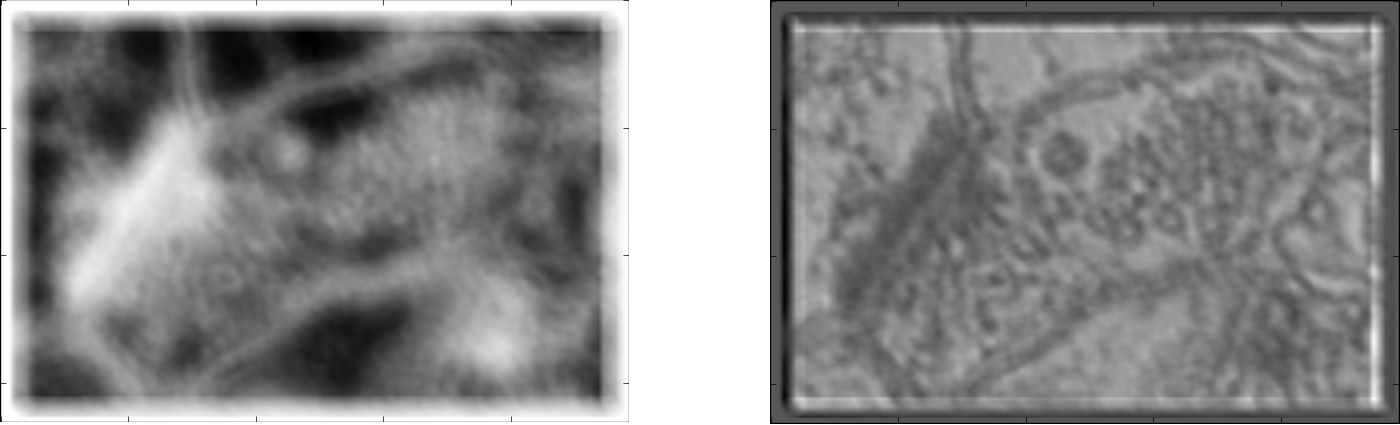
\includegraphics[scale=0.35]{files/premethod/img/convolve_edge.png}
	\caption{Billeder foldet med matricer. Venstre billede med matrice med 0 i indre. Højre billede med matrice med 10 i indre.\label{fig:premethod_vesEdgeConv}}
\end{figure}

Billederne er meget forskellige, så det er tydeligt at det har en stor betydning med hvilke tal der vælges til hver indgang. I det venstre billede er der svært at se en eneste vesikel, hvorimod den højre er væsentlig tydeligere. Dette resultat er et skridt i den rigtige retning da vi nu begynder at kunne se flere af vesiklerne. Der er dog stadig problemer i venstre side af cellen hvor overgangen mellem vesiklerne er svær at se.

%% Kildeangivelser:
% http://en.wikipedia.org/w/index.php?title=Image_gradient&oldid=421160257
% http://en.wikipedia.org/w/index.php?title=Gaussian_blur&oldid=422700764
% http://en.wikipedia.org/w/index.php?title=Sobel_operator&oldid=422155717
% http://en.wikipedia.org/w/index.php?title=Hough_transform&oldid=422150042
% http://en.wikipedia.org/w/index.php?title=Canny_edge_detector&oldid=421218460
% http://en.wikipedia.org/w/index.php?title=Edge_detection&oldid=425584110
% http://en.wikipedia.org/w/index.php?title=Difference_of_Gaussians&oldid=418426534
